\chapter{Antecedentes}
\label{chap:antec}

La frecuencia es la magnitud que mide la cantidad de pulsos que ocurren en un instante de tiempo. Determina la cantidad de latidos del coraz\'on o el {\em tempo}\footnote{El {\em tempo} es la velocidad con la que se ejecuta una pieza musical.} musical; ambos medidos en {\em pulsos por minuto} (bpm, del ingl\'es {\em beats per minute}). Para determinar la frecuencia en una onda es necesario saber cu\'al es su longitud de onda. La longitud de onda se determina por la distancia entre dos {\em crestas}\footnote{La {\em cresta} es el punto m\'as alto de una onda.} o dos {\em valles}\footnote{El {\em valle} es el punto m\'as bajo de una onda.} consecutivos.

\noindent La figura \ref{fig:freq} muestra un ejemplo de gr\'afica de una onda cuya frecuencia disminuye con el progreso del tiempo.

\begin{figure}[h!]
\begin{center}
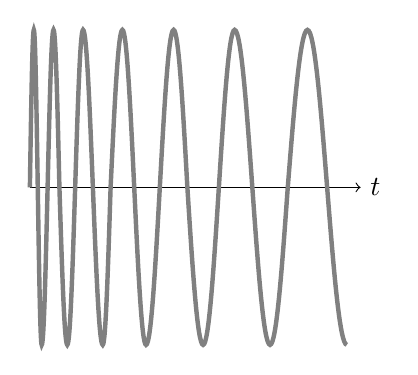
\begin{tikzpicture}
\shorthandoff{<>."}
  \draw[->] (0,0) -- (4.2,0) node[right] {$t$};
  \draw [x=0.5cm,y=2cm, ultra thick, gray] (0,0) 
  sin (0.1,1) cos (0.2,0) sin (0.3,-1) 
  cos (0.45,0) sin (0.6,1) cos (0.75,0) 
  sin (0.95,-1) cos (1.15,0) sin (1.35,1)
  cos (1.6,0) sin (1.85,-1) cos (2.05,0) 
  sin (2.35,1) cos (2.65,0) sin (2.95,-1)
  cos (3.3,0) sin (3.65,1) cos (4,0)
  sin (4.4,-1) cos (4.8,0) sin (5.2,1)
  cos (5.65,0) sin (6.1,-1) cos (6.55,0)
  sin (7.05,1) cos (7.55,0) sin (8.05,-1);
  \shorthandon{<>."}
\end{tikzpicture}
\end{center}
\caption[Frecuencia mayor a menor]{La onda disminuye su frecuencia con la progresi\'on de tiempo $t$.}
\label{fig:freq}
\end{figure}

\noindent \citet{StevenAudio} menciona que el o\'ido humano es un \'organo sumamente complejo. Es sensible a la vibraci\'on de las ondas mec\'anicas producidas a cierta frecuencia. Espec\'ificamente el umbral de audici\'on va desde los 20Hz hasta los 20kHz. El o\'ido es menos sensible a frecuencias m\'as bajas o m\'as altas a las anteriores.

\noindent La {\em c\'oclea} es una estructura interna del o\'ido llena del l\'iquido por el cual viajan las ondas recibidas, solo una porci\'on de las ondas logran pasar y estimulan el nervio auditivo. De esta manera podemos oir.

%\section{Conceptos generales}

\noindent Los sonidos que se reproducen en la computadora o en cualquier otro dispositivo electr\'onico est\'an preparados para el o\'ido humano. Al procesar el sonido se filtran las frecuencias no audibles, de esta manera se ahorra espacio, tambi\'en se procesa el sonido a una velocidad tal que los fragmentos de la pista de sonido no produzcan silencios.

\noindent Generalmente estos fragmentos son almacenados en archivos los cuales son tratados de alguna manera para reproducirlos. Estos archivos contienen informaci\'on b\'asica que indica la forma en que se reproducir\'a el sonido, como el n\'umero de fragmentos de sonido en el archivo o la cantidad de fragmentos que se reproducen por segundo. El archivo tambi\'en contiene los datos del sonido a reproducir comprimidos en alg\'un formato que el reproductor puede interpretar.

\noindent Para reproducir un sonido en alg\'un dispositivo electr\'onico se lleva a cabo una serie de procesos algor\'itmicos que sirven para interpretar los datos almacenados en los archivos, algo conocido como {\em decodificaci\'on}. Una vez decodificados los datos se obtiene informaci\'on que describe una {\em onda ac\'ustica} \cite{izaguirre2008sistemas}.

\noindent Cuando se reproduce un sonido lo que en realidad se escucha es una representaci\'on del sonido real, que ha sido procesada. La onda que se reproduce puede ser muy similar pero no igual al sonido original. Este sonido producido es conocido como {\em sonido digital}.

\section{Procesamiento de se\~nales}

La producci\'on de sonido digital es un proceso de transformaci\'on de una se\~nal anal\'ogica a digital. \citet{Baher} describe tres etapas:

\begin{description}
\item[Muestreo.]{El proceso en el que una se\~nal anal\'ogica es transformada en {\em datos discretizados}.}
\item[Cuantificaci\'on.]{Es la {\em digitalizaci\'on} de los datos obtenidos durante el muestreo de la se\~nal.}
\item[Codificaci\'on.]{El proceso de almacenado de la se\~nal discretizada en alg\'un formato de {\em codec}.}
\end{description}

\noindent Estas tres etapas se discuten en detalle a continuaci\'on.

\subsection{Muestreo}

Para poder trabajar con sonidos digitales, es necesario reducir las se\~nales deben a muestras discretas de un dominio de tiempo discreto. Esta operaci\'on es llamada {\em muestreo}.

\noindent El muestreo consiste en tomar valores de una se\~nal de tiempo continuo en instantes de tiempo m\'ultiplos de $T$, llamado intervalo de muestreo. La cantidad $F_s = 1/T$ es llamada {\em frecuencia de muestreo} \cite{Davide}. En la figura \ref{fig:muest} se ilustra un ejemplo del proceso de muestreo.

\begin{figure}[h!]
\centering
\begin{minipage}[c][5cm][t]{.5\textwidth}
\centering
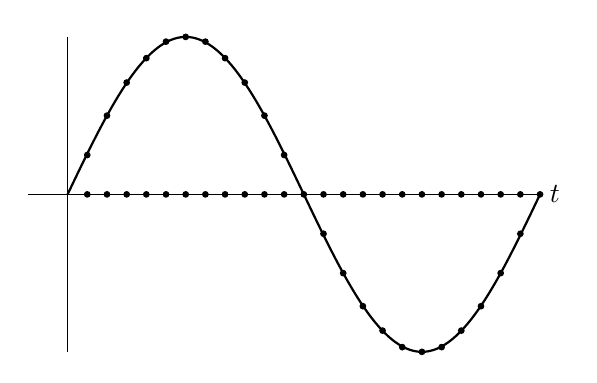
\begin{tikzpicture}
\shorthandoff{<>."}
  \draw[-] (-.5,0) -- (6,0) node[right] {$t$};
  \draw[-] (0,-2) -- (0,2) node[right] {$$};
  \draw [x=0.5cm,y=2cm, thick, black] (0,0) 
  sin (3,1) cos (6,0) sin (9,-1) cos (12,0);  
  \filldraw (0.25,0) circle (1pt);
  \filldraw (0.25,.5) circle (1pt);
  
  \filldraw (0.5,0) circle (1pt);
  \filldraw (0.5,1) circle (1pt);
  
  \filldraw (0.75,0) circle (1pt);
  \filldraw (0.75,1.42) circle (1pt);
  
  \filldraw (1,0) circle (1pt);
  \filldraw (1,1.73) circle (1pt);
    
  \filldraw (1.25,0) circle (1pt);
  \filldraw (1.25,1.94) circle (1pt);

  \filldraw (1.5,0) circle (1pt);
  \filldraw (1.5,2) circle (1pt);
  
  \filldraw (1.75,0) circle (1pt);
  \filldraw (1.75,1.94) circle (1pt);

  \filldraw (2,0) circle (1pt);
  \filldraw (2,1.73) circle (1pt);

  \filldraw (2.25,0) circle (1pt);
  \filldraw (2.25,1.42) circle (1pt);

  \filldraw (2.5,0) circle (1pt);
  \filldraw (2.5,1) circle (1pt);

  \filldraw (2.75,0) circle (1pt);
  \filldraw (2.75,.5) circle (1pt);

  \filldraw (3,0) circle (1pt);

  \filldraw (3.25,0) circle (1pt);
  \filldraw (3.25,-.5) circle (1pt);

  \filldraw (3.5,0) circle (1pt);
  \filldraw (3.5,-1) circle (1pt);

  \filldraw (3.75,0) circle (1pt);
  \filldraw (3.75,-1.42) circle (1pt);

  \filldraw (4,0) circle (1pt);
  \filldraw (4,-1.73) circle (1pt);

  \filldraw (4.25,0) circle (1pt);
  \filldraw (4.25,-1.94) circle (1pt);

  \filldraw (4.5,0) circle (1pt);
  \filldraw (4.5,-2) circle (1pt);

  \filldraw (4.75,0) circle (1pt);
  \filldraw (4.75,-1.94) circle (1pt);

  \filldraw (5,0) circle (1pt);
  \filldraw (5,-1.73) circle (1pt);

  \filldraw (5.25,0) circle (1pt);
  \filldraw (5.25,-1.42) circle (1pt);

  \filldraw (5.5,0) circle (1pt);
  \filldraw (5.5,-1) circle (1pt);

  \filldraw (5.75,0) circle (1pt);
  \filldraw (5.75,-.5) circle (1pt);

  \filldraw (6,0) circle (1pt);
  \shorthandon{<>."}
\end{tikzpicture}

\\a)
\end{minipage}%
\begin{minipage}[c][5cm][t]{.5\textwidth}
\centering
\begin{tikzpicture}
\shorthandoff{<>."}
  \draw[-] (-.5,0) -- (6,0) node[right] {$t$};
  \draw[-] (0,-2) -- (0,2) node[right] {$$};
  \draw (0.25,0) -- (0.25,.5);
  
  \draw (0.5,0) -- (0.5,1);
  
  \draw (0.75,0) -- (0.75,1.42);
  
  \draw (1,0) -- (1,1.73);
    
  \draw (1.25,0) -- (1.25,1.94);

  \draw (1.5,0) -- (1.5,2);
  
  \draw (1.75,0) -- (1.75,1.94);

  \draw (2,0) -- (2,1.73);

  \draw (2.25,0) -- (2.25,1.42);

  \draw (2.5,0) -- (2.5,1);

  \draw (2.75,0) -- (2.75,.5);

  \draw (3.25,0) -- (3.25,-.5);

  \filldraw (3.5,0) -- (3.5,-1);

  \filldraw (3.75,0) -- (3.75,-1.42);

  \filldraw (4,0) -- (4,-1.73);

  \filldraw (4.25,0) -- (4.25,-1.94);

  \filldraw (4.5,0) -- (4.5,-2);

  \filldraw (4.75,0) -- (4.75,-1.94);

  \filldraw (5,0) -- (5,-1.73);

  \filldraw (5.25,0) -- (5.25,-1.42);

  \filldraw (5.5,0) -- (5.5,-1);

  \filldraw (5.75,0) -- (5.75,-.5);

  \shorthandon{<>."}
\end{tikzpicture}

\\b)
\end{minipage}%
\caption[Proceso de muestreo]{En a) se toman muestras de una onda en intervalos de tiempo regulares $t$, en b) se hace una representaci\'on digital de la onda.}
\label{fig:muest}
\end{figure}

\subsection{Cuantificaci\'on}

Los datos obtenidos del muestreo ahora pueden ser representados como una se\~nal de tiempo discreto y valores continuos. Con la cuantificaci\'on los valores se discretizan. El valor de cada muestra es aproximado entonces con un valor de un conjunto finito de posibles valores. La diferencia entre el valor continuo y su aproximaci\'on se le denomina error de cuantificaci\'on \cite{Baher}. En la figura \ref{fig:cuant} se puede ver un ejemplo de cuantificaci\'on de una se\~nal.

\begin{figure}[h!]
\centering
\begin{minipage}[c][5cm][t]{.5\textwidth}
\centering
\begin{tikzpicture}
\shorthandoff{<>."}
  \draw[-] (-.5,0) -- (6,0) node[right] {$t$};
  \draw[-] (0,-2) -- (0,2) node[right] {$$};
  \draw (0.25,0) -- (0.25,.5);
  \draw (0.25,.5) -- (0.5,.5);

  \draw (0.5,.5) -- (0.5,1);
  \draw (0.5,1) -- (0.75,1);

  \draw (0.75,01) -- (0.75,1.42);
  \draw (0.75,1.42) -- (1,1.42);

  \draw (1,1.42) -- (1,1.73);
  \draw (1,1.73) -- (1.25,1.73);

  \draw (1.25,1.73) -- (1.25,1.94);
  \draw (1.25,1.94) -- (1.5,1.94);

  \draw (1.5,1.94) -- (1.5,2);
  \draw (1.5,2) -- (1.75,2);

  \draw (1.75,2) -- (1.75,1.94);
  \draw (1.75,1.94) -- (2,1.94);

  \draw (2,1.94) -- (2,1.73);
  \draw (2,1.73) -- (2.25,1.73);

  \draw (2.25,1.73) -- (2.25,1.42);
  \draw (2.25,1.42) -- (2.5,1.42);

  \draw (2.5,1.42) -- (2.5,1);
  \draw (2.5,1) -- (2.75,1);

  \draw (2.75,1) -- (2.75,.5);
  \draw (2.75,.5) -- (3,.5);

  \draw (3,.5) -- (3,0);
  \draw (3,0) -- (3.25,0);
  
  \draw (3.25,0) -- (3.25,-.5);
  \draw (3.25,-.5) -- (3.5,-.5);

  \draw (3.5,-.5) -- (3.5,-1);
  \draw (3.5,-1) -- (3.75,-1);
  
  \draw (3.75,-1) -- (3.75,-1.42);
  \draw (3.75,-1.42) -- (4,-1.42);
  
  \draw (4,-1.42) -- (4,-1.73);
  \draw (4,-1.73) -- (4.25,-1.73);

  \draw (4.25,-1.73) -- (4.25,-1.94);
  \draw (4.25,-1.94) -- (4.5,-1.94);

  \draw (4.5,-1.94) -- (4.5,-2);
  \draw (4.5,-2) -- (4.75,-2);

  \draw (4.75,-2) -- (4.75,-1.94);
  \draw (4.75,-1.94) -- (5,-1.94);

  \draw (5,-1.94) -- (5,-1.73);
  \draw (5,-1.73) -- (5.25,-1.73);

  \draw (5.25,-1.73) -- (5.25,-1.42);
  \draw (5.25,-1.42) -- (5.5,-1.42);

  \draw (5.5,-1.42) -- (5.5,-1);
  \draw (5.5,-1) -- (5.75,-1);

  \draw (5.75,-1) -- (5.75,-.5);
  \draw (5.75,-.5) -- (6,-.5);

  \draw (6,-.5) -- (6,0);

  \shorthandon{<>."}
\end{tikzpicture}

\\a)
\end{minipage}%
\begin{minipage}[c][5cm][t]{.5\textwidth}
\centering
\begin{tikzpicture}
\shorthandoff{<>."}
  \draw[-] (-.5,0) -- (6,0) node[right] {$t$};
  \draw[-] (0,-2) -- (0,2) node[right] {$$};
  \draw (0,0) -- (0.25,.5);
  \draw (0.25,.5) -- (0.5,1);

  \draw (0.5,1) -- (0.75,1.42);
  \draw (0.75,1.42) -- (1,1.73);

  \draw (1,1.73) -- (1.25,1.93);

  \draw (1.25,1.94) -- (1.5,2);

  \draw (1.5,2) -- (1.75,1.94);

  \draw (1.75,1.94) -- (2,1.73);

  \draw (2,1.73) -- (2.25,1.42);

  \draw (2.25,1.42) -- (2.5,1);

  \draw (2.5,1) -- (2.75,.5);

  \draw (2.75,.5) -- (3,0);

  \draw (3,0) -- (3.25,-.5);
  
  \draw (3.25,-.5) -- (3.5,-1);

  \draw (3.5,-1) -- (3.75,-1.42);
  
  \draw (3.75,-1.42) -- (4,-1.73);
  
  \draw (4,-1.73) -- (4.25,-1.94);

  \draw (4.25,-1.94) -- (4.5,-2);

  \draw (4.5,-2) -- (4.75,-1.94);

  \draw (4.75,-1.94) -- (5,-1.73);

  \draw (5,-1.73) -- (5.25,-1.42);

  \draw (5.25,-1.42) -- (5.5,-1);

  \draw (5.5,-1) -- (5.75,-.5);

  \draw (5.75,-.5) -- (6,0);

  \shorthandon{<>."}
\end{tikzpicture}

\\b)
\end{minipage}%
\caption[Proceso de cuantificaci\'on]{La representaci\'on digital es discretizada en a) y posteriormente se suavizan los valores de \'esta en b) para dar una forma parecida a la onda original.}
\label{fig:cuant}
\end{figure}

\subsection{Codificaci\'on}

Despu\'es de la cuantificaci\'on se tiene una se\~nal de timepo discreto con valores discretos como la de la figura \ref{fig:cod1} que se puede almacenar en un {\em contenedor}; este contenedor comprime la informaci\'on mediante alg\'un algoritmo de codificaci\'on, puede ser con o sin p\'erdida. La compresi\'on con p\'erdida usa algoritmos que almacenan una se\~nal similar pero no igual a la original. La compresi\'on sin p\'erdida usa un algoritmo que almacena los datos originales, generalmente ocupan una cantidad de espacio en disco mayor \cite{StevenAudio}.

\begin{figure}[h!]
\begin{center}
\scalebox{1.6}{
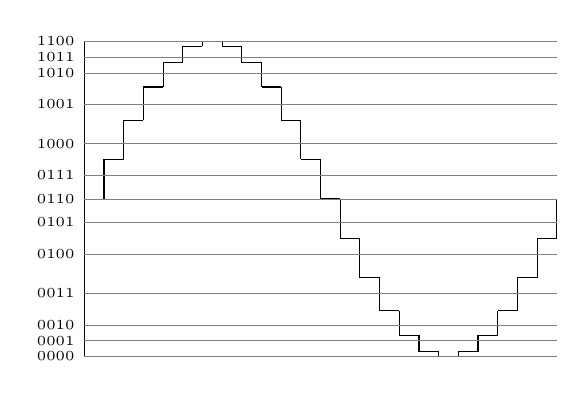
\begin{tikzpicture}
\shorthandoff{<>."}
  \draw[-] (0,-2) -- (0,2) node[right] {$$};
  \draw (0.25,0) -- (0.25,.5);
  \draw (0.25,.5) -- (0.5,.5);

  \draw (0.5,.5) -- (0.5,1);
  \draw (0.5,1) -- (0.75,1);

  \draw (0.75,01) -- (0.75,1.42);
  \draw (0.75,1.42) -- (1,1.42);

  \draw (1,1.42) -- (1,1.73);
  \draw (1,1.73) -- (1.25,1.73);

  \draw (1.25,1.73) -- (1.25,1.94);
  \draw (1.25,1.94) -- (1.5,1.94);

  \draw (1.5,1.94) -- (1.5,2);
  \draw (1.5,2) -- (1.75,2);

  \draw (1.75,2) -- (1.75,1.94);
  \draw (1.75,1.94) -- (2,1.94);

  \draw (2,1.94) -- (2,1.73);
  \draw (2,1.73) -- (2.25,1.73);

  \draw (2.25,1.73) -- (2.25,1.42);
  \draw (2.25,1.42) -- (2.5,1.42);

  \draw (2.5,1.42) -- (2.5,1);
  \draw (2.5,1) -- (2.75,1);

  \draw (2.75,1) -- (2.75,.5);
  \draw (2.75,.5) -- (3,.5);

  \draw (3,.5) -- (3,0);
  \draw (3,0) -- (3.25,0);
  
  \draw (3.25,0) -- (3.25,-.5);
  \draw (3.25,-.5) -- (3.5,-.5);

  \draw (3.5,-.5) -- (3.5,-1);
  \draw (3.5,-1) -- (3.75,-1);
  
  \draw (3.75,-1) -- (3.75,-1.42);
  \draw (3.75,-1.42) -- (4,-1.42);
  
  \draw (4,-1.42) -- (4,-1.73);
  \draw (4,-1.73) -- (4.25,-1.73);

  \draw (4.25,-1.73) -- (4.25,-1.94);
  \draw (4.25,-1.94) -- (4.5,-1.94);

  \draw (4.5,-1.94) -- (4.5,-2);
  \draw (4.5,-2) -- (4.75,-2);

  \draw (4.75,-2) -- (4.75,-1.94);
  \draw (4.75,-1.94) -- (5,-1.94);

  \draw (5,-1.94) -- (5,-1.73);
  \draw (5,-1.73) -- (5.25,-1.73);

  \draw (5.25,-1.73) -- (5.25,-1.42);
  \draw (5.25,-1.42) -- (5.5,-1.42);

  \draw (5.5,-1.42) -- (5.5,-1);
  \draw (5.5,-1) -- (5.75,-1);

  \draw (5.75,-1) -- (5.75,-.5);
  \draw (5.75,-.5) -- (6,-.5);

  \draw (6,-.5) -- (6,0);

\node[left] at (0,-2)	{\tiny 0000};
\node[left] at (0,-1.8)	{\tiny 0001};
\node[left] at (0,-1.6)	{\tiny 0010};
\node[left] at (0,-1.2)	{\tiny 0011};
\node[left] at (0,-.7)	{\tiny 0100};
\node[left] at (0,-.3)	{\tiny 0101};
\node[left] at (0,0)	{\tiny 0110};
\node[left] at (0,.3)	{\tiny 0111};
\node[left] at (0,.7)	{\tiny 1000};
\node[left] at (0,1.2)	{\tiny 1001};
\node[left] at (0,1.6)	{\tiny 1010};
\node[left] at (0,1.8)	{\tiny 1011};
\node[left] at (0,2)	{\tiny 1100};

\draw[-,gray,very thin] (0,2) -- (6,2);
\draw[-,gray,very thin] (0,1.8) -- (6,1.8);
\draw[-,gray,very thin] (0,1.6) -- (6,1.6);
\draw[-,gray,very thin] (0,1.2) -- (6,1.2);
\draw[-,gray,very thin] (0,.7) -- (6,.7);
\draw[-,gray,very thin] (0,.3) -- (6,.3);
\draw[-,gray,very thin] (0,0) -- (6,0);
\draw[-,gray,very thin] (0,-.3) -- (6,-.3);
\draw[-,gray,very thin] (0,-.7) -- (6,-.7);
\draw[-,gray,very thin] (0,-1.2) -- (6,-1.2);
\draw[-,gray,very thin] (0,-1.6) -- (6,-1.6);
\draw[-,gray,very thin] (0,-1.8) -- (6,-1.8);
\draw[-,gray,very thin] (0,-2) -- (6,-2);



  \shorthandon{<>."}
\end{tikzpicture}
}
\end{center}
\caption[Representaci\'on de una se\~nal cuantificada]{La se\~nal cuantificada puede representarse en forma de datos discretizados.}
\label{fig:cod1}
\end{figure}


\noindent Independientemente del metodo de compresi\'on, con la codificaci\'on se obtiene la informaci\'on de la se\~nal en un formato binario como se muestra en la figura \ref{fig:cod}.

\begin{figure}[h!]
\begin{center}
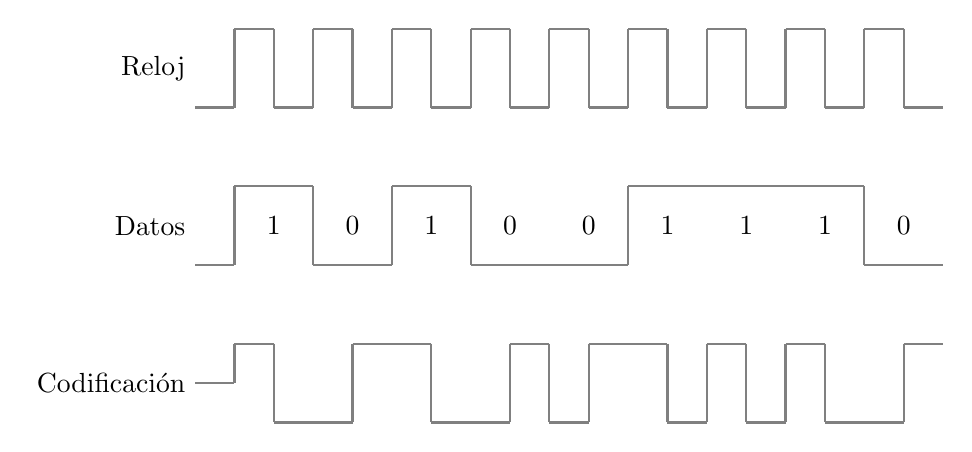
\begin{tikzpicture}
\shorthandoff{<>."}
\draw[thick,gray] (0,2) -- (0.5,2);
\draw[thick,gray] (0.5,2) -- (0.5,3);
\draw[thick,gray] (0.5,3) -- (1,3);
\draw[thick,gray] (1,3) -- (1,2);
\draw[thick,gray] (1,2) -- (1.5,2);
\draw[thick,gray] (1.5,2) -- (1.5,3);
\draw[thick,gray] (1.5,3) -- (2,3);
\draw[thick,gray] (2,3) -- (2,2);
\draw[thick,gray] (2,2) -- (2.5,2);
\draw[thick,gray] (2.5,2) -- (2.5,3);
\draw[thick,gray] (2.5,3) -- (3,3);
\draw[thick,gray] (3,3) -- (3,2);
\draw[thick,gray] (3,2) -- (3.5,2);
\draw[thick,gray] (3.5,2) -- (3.5,3);
\draw[thick,gray] (3.5,3) -- (4,3);
\draw[thick,gray] (4,3) -- (4,2);
\draw[thick,gray] (4,2) -- (4.5,2);
\draw[thick,gray] (4.5,2) -- (4.5,3);
\draw[thick,gray] (4.5,3) -- (5,3);
\draw[thick,gray] (5,3) -- (5,2);
\draw[thick,gray] (5,2) -- (5.5,2);
\draw[thick,gray] (5.5,2) -- (5.5,3);
\draw[thick,gray] (5.5,3) -- (6,3);
\draw[thick,gray] (6,3) -- (6,2);
\draw[thick,gray] (6,2) -- (6.5,2);
\draw[thick,gray] (6.5,2) -- (6.5,3);
\draw[thick,gray] (6.5,3) -- (7,3);
\draw[thick,gray] (7,3) -- (7,2);
\draw[thick,gray] (7,2) -- (7.5,2);
\draw[thick,gray] (7.5,2) -- (7.5,3);
\draw[thick,gray] (7.5,3) -- (8,3);
\draw[thick,gray] (8,3) -- (8,2);
\draw[thick,gray] (8,2) -- (8.5,2);
\draw[thick,gray] (8.5,2) -- (8.5,3);
\draw[thick,gray] (8.5,3) -- (9,3);
\draw[thick,gray] (9,3) -- (9,2);
\draw[thick,gray] (9,2) -- (9.5,2);

\node[left] at (0,2.5){Reloj};

\draw[thick,gray] (0,0) -- (0.5,0);
\draw[thick,gray] (0.5,0) -- (0.5,1);
\draw[thick,gray] (0.5,1) -- (1.5,1);
\draw[thick,gray] (1.5,1) -- (1.5,0);
\draw[thick,gray] (1.5,0) -- (2.5,0);
\draw[thick,gray] (2.5,0) -- (2.5,1);
\draw[thick,gray] (2.5,1) -- (3.5,1);
\draw[thick,gray] (3.5,1) -- (3.5,0);
\draw[thick,gray] (3.5,0) -- (5.5,0);
\draw[thick,gray] (5.5,0) -- (5.5,1);
\draw[thick,gray] (5.5,1) -- (8.5,1);
\draw[thick,gray] (8.5,1) -- (8.5,0);
\draw[thick,gray] (8.5,0) -- (9.5,0);

\node[left] at (0,0.5){Datos};
\node at (1,.5){1};
\node at (2,.5){0};
\node at (3,.5){1};
\node at (4,.5){0};
\node at (5,.5){0};
\node at (6,.5){1};
\node at (7,.5){1};
\node at (8,.5){1};
\node at (9,.5){0};

\draw[thick,gray] (0,-1.5) -- (0.5,-1.5);
\draw[thick,gray] (0.5,-1.5) -- (0.5,-1);
\draw[thick,gray] (0.5,-1) -- (1,-1);
\draw[thick,gray] (1,-1) -- (1,-2);
\draw[thick,gray] (1,-2) -- (2,-2);
\draw[thick,gray] (2,-2) -- (2,-1);
\draw[thick,gray] (2,-1) -- (3,-1);
\draw[thick,gray] (3,-1) -- (3,-2);
\draw[thick,gray] (3,-2) -- (4,-2);
\draw[thick,gray] (4,-2) -- (4,-1);
\draw[thick,gray] (4,-1) -- (4.5,-1);
\draw[thick,gray] (4.5,-1) -- (4.5,-2);
\draw[thick,gray] (4.5,-2) -- (5,-2);
\draw[thick,gray] (5,-2) -- (5,-1);
\draw[thick,gray] (5,-1) -- (6,-1);
\draw[thick,gray] (6,-1) -- (6,-2);
\draw[thick,gray] (6,-2) -- (6.5,-2);
\draw[thick,gray] (6.5,-2) -- (6.5,-1);
\draw[thick,gray] (6.5,-1) -- (7,-1);
\draw[thick,gray] (7,-1) -- (7,-2);
\draw[thick,gray] (7,-2) -- (7.5,-2);
\draw[thick,gray] (7.5,-2) -- (7.5,-1);
\draw[thick,gray] (7.5,-1) -- (8,-1);
\draw[thick,gray] (8,-1) -- (8,-2);
\draw[thick,gray] (8,-2) -- (9,-2);
\draw[thick,gray] (9,-2) -- (9,-1);
\draw[thick,gray] (9,-1) -- (9.5,-1);

\node[left] at (0,-1.5){Codificaci\'on};

\shorthandon{<>."}
\end{tikzpicture}
\end{center}
\caption[Proceso de codificaci\'on]{Proceso de codificaci\'on de una se\~nal transformada a datos.}
\label{fig:cod}
\end{figure}
\section {Transformada r\'apida de Fourier}

Durante el procesamiento de se\~nales puede ser de utilidad analizar frecuencias por separado. La {\em transformada r\'apida de Fourier} permite separar una se\~nal de onda en sus diferentes frecuencias. La figura \ref{fig:trans} muestra un ejemplo gr\'afico del funcionamiento del algoritmo.

\newcommand{\waves}[5][purple]{
\def\a{1+#3}
\def\b{#3}
\def\c{1-#3}
\def\x{#4}
\def\y{#5}
\foreach \val in {0,#3,...,#2}{
\def\i{\x+\val*4}
\def\var{\y+\val}
\draw[ultra thick, #1] (\i + \b*5,-1+\var) cos (\i + \b*4,0+\var); 
\draw[ultra thick, #1] (\i + \b*4,0+\var) sin (\i + \b*3,\a+\var); 
\draw[ultra thick, #1] (\i + \b*3,\a+\var) cos (\i + \b*2,\b+\var); 
\draw[ultra thick, #1] (\i + \b*2,\b+\var) sin (\i + \b,-\c+\var);}
}
\begin{figure}[h!]
\begin{center}
\scalebox{0.6}{
\begin{tikzpicture}
\waves[green]{1}{0.3}{-6}{3}
\waves[blue]{1}{0.2}{-4}{2}
\waves{1}{0.05}{-2}{1}
\waves{1}{0.05}{0}{0}
\waves[blue]{1}{0.2}{2}{-1}
\waves[green]{1}{0.3}{4}{-2}
\draw(-7, 1.5)--(4,-4);
\draw(4,-4)--(10,-2.5);

\node[right] at (4.5,-5){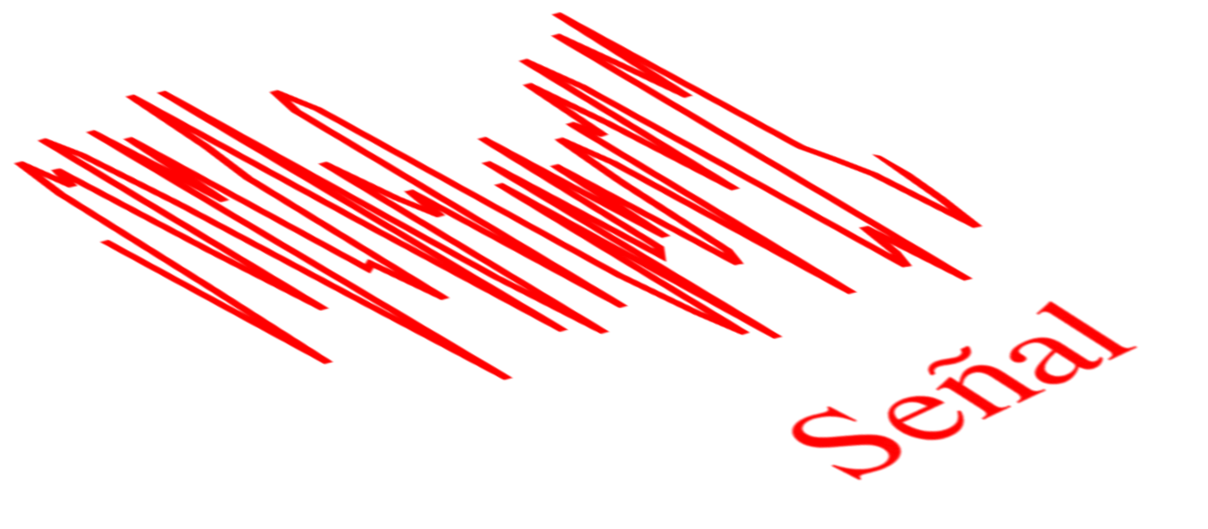
\includegraphics[height=35mm]{./Figuras/noise}};
\node[right] at (-10,-3.5){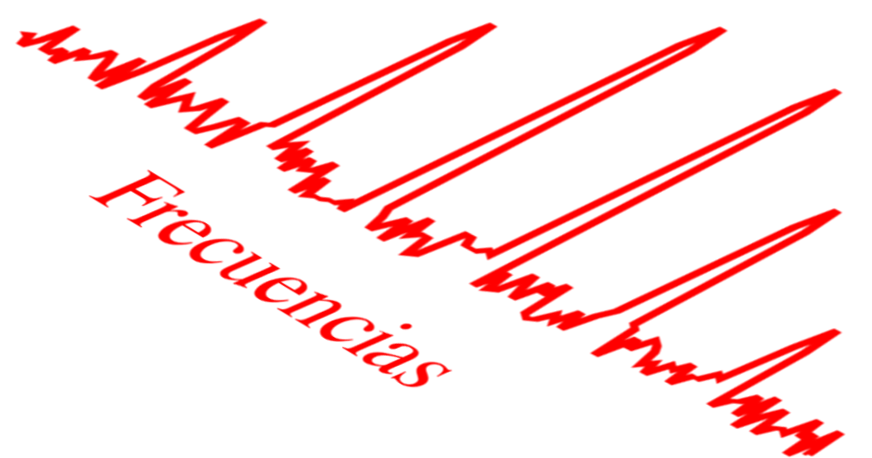
\includegraphics[height=50mm]{./Figuras/freq}};

\end{tikzpicture}}
\end{center}
\caption[Transformada de Fourier]{Comparaci\'on entre una se\~nal y sus frecuencias separadas en ondas individuales.}
\label{fig:trans}
\end{figure}

\noindent A continuaci\'on se describe uno de los algoritmos m\'as usados \cite{walker1996fast}. Se asume que $N = 2^R$ donde $R$ es un entero positivo:
\begin{equation}
H_{k} = \sum_{j=0}^{N-1}h_{j}W^{jk}, \text{donde } W = e^{\pm \frac{2\pi i}{N}}\
\end{equation}

\section{Reconocimiento de patrones}

El reconocimiento de patrones consiste en la extracci\'on de caracter\'isticas importantes en imagenes, sonidos, cadenas de ADN, etc\'etera. \citet{Satosi} menciona que un patr\'on es una entidad, vagamente definida, la cual puede nombrarse.

\noindent \citet{Kittler} en sus notas de seminario menciona que es posible modelar un sistema de tres estados basado en el sistema perceptual de un ser humano:

\begin{description}
\item [Adquisici\'on de datos.] {Consiste en recolectar informaci\'on de alg\'un medio ya sea una c\'amara, un micr\'ofono, o cualquier sensor que genere datos en bruto.}
\item [Extracci\'on de caracter\'isticas.] {Mediante el uso de algoritmos tratar de encontrar informaci\'on relevante dentro de los datos adquiridos.}
\item [Toma de desiciones.] {Cuando se tienen las caracter\'isticas relevantes ahora se clasifican dependiendo del prop\'osito del programa.}
\end{description}

\noindent Existen diferentes aproximaciones a este problema, a continuaci\'on se describen brevemente alg\'unas de la m\'as utilizadas \cite{Anil}.

\begin{description}

\item[Comparaci\'on de plantillas]{Este es el modelo m\'as sencillo y quiz\'a uno de los primeros en existir. Consiste en comparar una plantilla con la informaci\'on de una muestra obtenida buscando similitudes}
\item[Modelo estad\'istico]{Este modelo se basa en la teor\'ia de probabilidad y estad\'istica y supone que se tiene un conjunto de medidas num\'ericas con distribuciones de probabilidad conocidas y a partir de ellas se realiza el reconocimiento.}
\item[Modelo sint\'actico]{Este modelo se basa en encontrar las relaciones estructurales que guardan los objetos de estudio, utilizando la teor\'ia de lenguajes formales. El objetivo es construir una gram\'atica que describa la estructura del universo de objetos.}
\item[Redes neuronales]{Este modelo supone que tiene una estructura de neuronas interconectadas que se estimulan unas a otras, las cuales pueden ser ``entrenadas'' para dar una cierta respuesta cuando se le presentan determinados valores.}

\end{description}